\section{偏序格}
设\(\opair{L,\leq}\)是偏序集,\(\leq\)是\(L\)上的偏序关系,
\(L\)中的两个元素的上确界及下确界不一定存在.
例如,由哈斯图 \labelcref{figure:格论.偏序集1} 可知,
\(\{c,b\}\)无上确界,\(\{a,d\}\)无下确界.

\begin{figure}[htb]
%@see: 《离散数学》(邓辉文) P155 图5-1
	\centering
	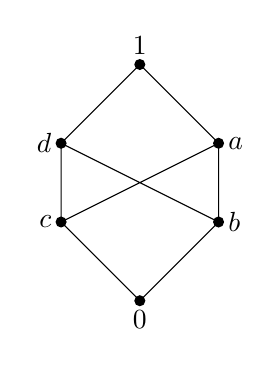
\begin{tikzpicture}
		\fill(0,0)circle(2pt);
		\fill(1,-1)circle(2pt);
		\fill(1,-2)circle(2pt);
		\fill(-1,-1)circle(2pt);
		\fill(-1,-2)circle(2pt);
		\fill(0,-3)circle(2pt);
		\draw(0,0)node[above]{$1$}
			--(1,-1)node[right]{$a$}
			--(1,-2)node[right]{$b$}
			--(0,-3)node[below]{$0$}
			--(-1,-2)node[left]{$c$}
			--(-1,-1)node[left]{$d$}--(0,0)
			(-1,-1)--(1,-2) (1,-1)--(-1,-2);
	\end{tikzpicture}
	\caption{}
	\label{figure:格论.偏序集1}
\end{figure}

\begin{definition}
%@see: 《离散数学》(邓辉文) P155 定义5-19
设\(\opair{L,\leq}\)是偏序集.
若\(L\)中任意两个元素都存在上确界和下确界,
则称\(\opair{L,\leq}\)是\DefineConcept{偏序格}(lattice).
%TODO 缺少定义:偏序集中任意两个元素的上确界、下确界
%@see: https://mathworld.wolfram.com/Lattice.html
\end{definition}

\begin{example}
%@see: 《离散数学》(邓辉文) P155 例5-27
设\(X\)是非空集合.
证明:\(\opair{\Powerset X,\subseteq}\)是偏序格.
\begin{proof}
显然\(\opair{\Powerset X,\subseteq}\)是偏序集.
对于任意\(A,B \in \Powerset X\),有\[
	\sup\{A,B\}
	= A \cup B
	\in \Powerset X,
	\qquad
	\inf\{A,B\}
	= A \cap B
	\in \Powerset X,
\]
所以\(\opair{\Powerset X,\subseteq}\)是偏序格.
\end{proof}
\end{example}

\begin{example}
%@see: 《离散数学》(邓辉文) P155
设\(A,B\)都是非空集合,
\(R\)是\(A\)与\(B\)的笛卡尔乘积\(A \times B\).
证明:\(\opair{R,\subseteq}\)是偏序格.
%TODO proof
% \begin{proof}
% 显然\(\opair{R,\subseteq}\)是偏序集.
% 对于任意\(x,y \in R\),有\[
% 	\sup\{x,y\}
% 	=
% \]
% \end{proof}
\end{example}

\begin{example}
%@see: 《离散数学》(邓辉文) P155 例5-28
设\(D_n\)是正整数\(n\)的全体正因数,即\[
	D_n = \Set{ x\in\mathbb{N}^+ \given x \mid n }.
\]
证明:\(\opair{D_n,\mid}\)是偏序格.
\begin{proof}
显然\(\opair{D_n,\mid}\)是偏序集.
对于任意\(x,y \in D_n\),有\[
	\sup\{x,y\}
	= \lcm{x,y}
	\in D_n,
	\qquad
	\inf\{x,y\}
	= \gcd{x,y}
	\in D_n,
\]
所以\(\opair{D_n,\mid}\)是偏序格.
\end{proof}
\end{example}

\begin{example}
%@see: 《离散数学》(邓辉文) P155 例5-29
设\(F\)是全体合式公式,\(\implies\)是逻辑蕴含关系.
证明:\(\opair{F,\implies}\)是偏序格.
\begin{proof}
显然\(\opair{F,\implies}\)是偏序集.

对于任意\(A,B \in F\),
由于\(A \implies A \lor B,
B \implies A \lor B\),
于是\(A \lor B\)是\(\{A,B\}\)的上界.
如果\(A \implies C,
B \implies C\),
那么\(A \lor B \implies C\),
所以\(\sup\{A,B\}
= A \lor B
\in F\).

对于任意\(A,B \in F\),
因为\(A \land B \implies A,
A \land B \implies B\),
于是\(A \land B\)是\(\{A,B\}\)的下界.
如果\(C \implies A,
C \implies B\),
那么\(C \implies A \land B\),
所以\(\inf\{A,B\}
= A \land B
\in F\).
\end{proof}
\end{example}

\begin{definition}
%@see: 《离散数学》(邓辉文) P156 定义5-20
设\(\opair{L,\leq}\)是偏序格.
对于任意\(x,y \in L\),
定义二元代数运算\begin{gather*}
	x + y \defeq \sup\{x,y\}, \\
	x \cdot y \defeq \inf\{x,y\}.
\end{gather*}
把\(+\)称为\DefineConcept{求上确界运算}.
%@see: https://mathworld.wolfram.com/Join.html
把\(\cdot\)称为\DefineConcept{求下确界运算}.
%@see: https://mathworld.wolfram.com/Meet.html
\end{definition}

\begin{theorem}
%@see: 《离散数学》(邓辉文) P156 定理5-7
设\(\opair{L,\leq}\)是偏序格,
则对于任意\(x,y \in L\)有\begin{gather*}
	x \leq x + y, \\
	y \leq x + y, \\
	x \cdot y \leq x, \\
	x \cdot y \leq y.
\end{gather*}
%TODO proof 下界 <= 下确界 <= 上确界 <= 上界
\end{theorem}

\begin{proposition}
%@see: 《离散数学》(邓辉文) P156
设\(\opair{L,\leq}\)是偏序格,
\(\geq\)是\(\leq\)的逆,
则\(\opair{L,\geq}\)也是偏序格.
\end{proposition}

应该注意到,\(\opair{L,\leq}\)和\(\opair{L,\geq}\)具有对称性,
\(\opair{L,\leq}\)中任意两个元素的上确界
就是相同元素在\(\opair{L,\geq}\)中的下确界,
\(\opair{L,\geq}\)中任意两个元素的下确界
就是相同元素在\(\opair{L,\leq}\)中的上确界,
即\[
	\sup_{\opair{L,\leq}}\{x,y\}
	= \inf_{\opair{L,\geq}}\{x,y\},
	\qquad
	\inf_{\opair{L,\leq}}\{x,y\}
	= \sup_{\opair{L,\geq}}\{x,y\}.
\]
若\(\opair{L,\leq}\)存在最大元素(记为\(1\)),则\(\opair{L,\geq}\)有最小元素(记为\(0\));
若\(\opair{L,\leq}\)存在最小元素\(0\),则\(\opair{L,\geq}\)有最大元素\(1\).
